\chapter{Building a data set for Comparative Argument Mining}
\label{sec:prestudy}
Due to the novelty of Argument Mining (and especially Comparative Argument Mining), the supply of data sets is small. Thus, a new data set had to be created.

This data set was designed to answer two questions: if a given sentence compares two known objects, and if it does, if the first-mentioned object is better or worse than the second one. Those questions will be translated to several classification tasks in the later chapters.

The data set was created using the crowdsourcing platform CrowdFlower\footnote{https://www.crowdflower.com (23.02.2018)}. As described in detail in the following chapters, the annotators were asked to assign one of four (and later three) classes to a sentence in which the objects of interest are highlighted.

The final data set contains 7421 sentences, each containing one of 273 object pairs. Each sentence was at least annotated by three different annotators.

\section{Common Crawl Text Corpus}
The sentences for the crowdsourcing task were obtained from a CommonCrawl\footnote{https://commoncrawl.org (23.02.2018)} data set. CommonCrawl is a non-profit organisation which crawls the web and releases the crawled data for free use.

The data\footnote{Download Link} used in this thesis was already preprocessed (see \cite{Panchenko:2017aa}). First, it contains only English text. Duplicates and near-duplicates were removed, as well as all HTML tags. The texts were then split into sentences.

The preprocessed sentences were used to obtain the sentences for the crowdsourcing task. To make them manageable, an ElasticSearch index (from now on called "the index") was created. The index contains 3,288,963,864 unique sentences.

To get an idea if there are enough comparative sentences in the index, it was queried for all sentences containing one of the words \enquote{\emph{better}} or \enquote{\emph{worse}},  as those words often indicate a comparison. This query returns 32,946,247 matching sentences. Querying for \enquote{\emph{is better than}} still returns 428,932 sentences.

Those numbers show that there are enough sentences in the index to create a dataset for the given task. Even if only 1\% of the sentences containing \enquote{\emph{is better than}} are truly comparative, there would be 4289 training examples for the machine learning algorithm using this query.


\section{Prestudies}
Before the main crowdsourcing task could start, several questions had to be answered:
\begin{enumerate}
\item How to extract sentences from the index? (How should the query look like?)
\item How to preprocress those sentences? (How to highlight the objects of interest?)
\item Which classes should be assigned to the sentences?
\item How to phrase the guidelines?
\end{enumerate}

Two prestudies were conducted to answer those questions.



\subsection{Sentence Selection}
The sentences for the crowdsourcing task should have a high probability of being comparative so that enough positive examples for the machine learning part are present. To ensure this, a list of cue words which indicate comparison was compiled by hand. For the prestudy, those words were \enquote{\emph{better}}, \enquote{\emph{worse}}, \enquote{\emph{inferior}}, \enquote{\emph{superior}}, and \enquote{\emph{because}}. Comparable objects are needed as well. A list of object pairs was selected by hand (see table \ref{tbl:prestudy-objects}). The pairs were selected in a way that they span a wide range of different domains, such as programming languages, countries and pets. The idea behind this is that pets are compared differently than programming languages. In this way, there will be different comparison patterns in the data.

\begin{table}[h]
\centering
\caption{Objects of the Annotation Prestudy}
\label{tbl:prestudy-objects}
\begin{tabular}{@{}llrrr@{}}
\toprule
First Object & Second Object      & \# Sentences                             \\ \midrule
Ruby    & Python    & 100      \\
BMW    & Mercedes    & 100  \\
USA & Europe & 100 \\
Beef & Chicken & 100   \\
Android & iPhone    &   100  \\
Cat & Dog      &     100  \\ 
Football & Baseball   &  100 \\ 
Wine & Beer  & 100  \\
Car & Bicycle & 100 \\
Summer & Winter &  100\\
\bottomrule  
                               
\end{tabular}
\end{table}

However, not all comparisons will contain one of the cue words mentioned above. Two different queries were used to overcome the coverage problem. Sevenhundred-fiftey sentences were obtained using query \ref{lst:es-query-a} (seventy-five for each pair) and 250 using query \ref{lst:es-query-b} (twenty-five for each pair). The second query will also match not-anticipated sentences such as \enquote{\emph{I like X more than Y since Z.}}.



\begin{lstlisting}[label=lst:es-query-a,breaklines=true,postbreak=\mbox{\textcolor{red}{$\hookrightarrow$}\space},caption=Prestudy Sentence Selection Query A]
{
  "query":{
    "bool":{
      "must":[
        {
          "query_string":{
            "default_field":"text",
            "query":"(better OR worse OR superior OR inferior OR because) AND \"<OBJECT_A>\" AND \"<OBJECT_B>\""
          }
        }
      ]
    }
  }
}
\end{lstlisting}

\begin{lstlisting}[label=lst:es-query-b,breaklines=true,postbreak=\mbox{\textcolor{red}{$\hookrightarrow$}\space},caption=Prestudy Sentence Selection Query B (shortened)]
[...]
          "query_string":{
            "default_field":"text",
            "query":" \"<OBJECT_A>\" AND \"<OBJECT_B>\""
[...]
\end{lstlisting}

Table \ref{tbl:example_sentences} shows some sentences obtained with this method. The objects of interest are printed in italics.

\begin{table}[h]
\centering
\caption{Extracted Sentences}
\label{tbl:example_sentences}
\begin{tabular}{@{}llr@{}}
\toprule
 Sentence   &  Cue Words Used                      \\ \midrule
 He's the best pet that you can get, Better than a \emph{dog} or \emph{cat}. & Yes \\
\emph{Android} phones have better processing power than \emph{iPhone} & Yes \\
 10 Things \emph{Android} Does Better Than \emph{iPhone} OS & Yes \\
 \emph{Dog} scared of \emph{cat} & No \\
 In fact, many 'supercars' will use \emph{BMW} or \emph{Mercedes} engines. & No \\

\bottomrule  
                               
\end{tabular}
\end{table}



\subsection{Prestudy A}
The first prestudy had two goals. First, it should assess if the sentence selection method returns enough comparative sentences. Second, the design of the study as described below should be checked. On that account, a crowdsourcing task with one hundred of the 1000 sentences was started.



For each sentence, the annotators should decide to which class a sentence belongs. The classes are described in table \ref{tbl:prestudyclasses-a}. The classes \texttt{BETTER}, \texttt{WORSE} and \texttt{NO\_COMP} directly refer to the questions stated at the beginning of chapter \ref{sec:prestudy}. The class \texttt{UNCLEAR} was added to capture all sentences which are in a way comparative but do not fit into the classes \texttt{BETTER} or \texttt{WORSE}.

\begin{figure}[h]
\centering
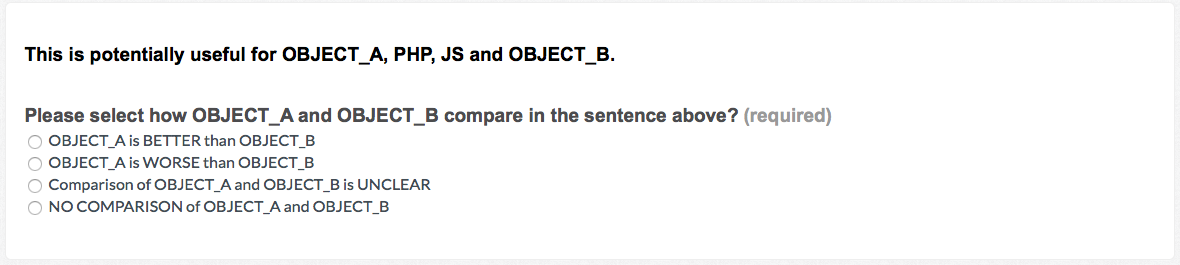
\includegraphics[width=1\textwidth]{images/prestudy/1_question}
\label{img:1_question}
\caption{Annotator view (Prestudy A)}
\end{figure}

\begin{table}[h]
\centering
\caption{Classes for Prestudy A and B}
\label{tbl:prestudyclasses-a}
\begin{tabular}{@{}ll@{}}
\toprule
Class & Description \\ \midrule
\texttt{BETTER} & The first object in the sentence (\texttt{OBJECT\_A}) is better than the second one (\texttt{OBJECT\_B})\\
\texttt{WORSE} & The first object is worse \\
\texttt{UNCLEAR} & Neither \texttt{BETTER} nor \texttt{WORSE} fits, but the sentence is comparative\\
\texttt{NO\_COMP} & The sentence is not comparative or the sentence is a question\\
\bottomrule
\end{tabular}
\end{table}

In each sentence, the first object of interest was replaced with \texttt{OBJECT\_A}, while the second one was replaced with \texttt{OBJECT\_B}. Table \ref{tbl:pre_1_res} shows examples of processed sentences. The idea behind this was to enable the annotators to quickly see which objects should be taken into account for assigning a class. For example, in sentence three of table \ref{tbl:pre_1_res}, the annotator might be confused which of the objects are of interest, yet the replacement makes it clear that he should ignore \enquote{\emph{C}} and \enquote{\emph{VB}}. The view of the annotator (for a single sentence) is shown in figure \ref{img:1_question}.

Each annotator saw five sentences to annotate per page. He was also able to look into the annotation guidelines anytime he wanted. To filter out low-quality annotators, twelve sentences were selected as test questions. Each participant took a quiz (eight test questions) before the actual annotation process. One of the five sentences on the page was a test question as well. The annotator had to keep an accuracy of 70\% on the test questions, otherwise he was removed from the task.

Figure \ref{fig:dist_pre_a} shows the class distribution of the annotation results. The numbers after the class names show the absolute members of that class. As 45\% of the sentences are comparative, the selection procedure works satisfying.

\begin{figure}[h]
\centering
\caption{Class Distribution (Prestudy A)}
\label{fig:dist_pre_a}
\begin{tikzpicture}
\pie [rotate=180, text = legend, color= {cgray, cgreen, cred, cblue}]
    {55/NO\_COMP (55),
    15/BETTER (15),
    8/WORSE (8),
    22/UNCLEAR (22)}
\end{tikzpicture}
\end{figure}

The agreement of the annotators was acceptable (see table \ref{fig:pre_a_agg}).

\begin{table}[h]
\caption{Agreement (Prestudy A)}
\label{fig:pre_a_agg}
\begin{tabularx}{\textwidth}{XXX}
\toprule
Distinct classes & Sentences & Percentage \\
\midrule
1 & 37 & 37.00\%\\
2 & 58 & 58.00\%\\
3 & 5 & 5.00\%\\
\bottomrule
\end{tabularx}
\end{table}


\begin{table}[h]
\centering
\caption{Uncertain Sentences (Prestudy A)}
\label{tbl:pre_1_res}
\begin{tabularx}{\textwidth}{lXrrr}
\toprule
\# & Sentence        & Ann. 1  & Ann. 2 & Ann. 3             \\ \midrule
1 & The only reason OBJECT\_A is used over OBJECT\_B, is because of libraries... & WORSE & UNCLEAR & NO\_COMP\\
2 & Agile development is the most popular model at the moment because of architectures like OBJECT\_A on Rails and Django (for OBJECT\_B) & NO\_COMP & NO\_COMP & UNCLEAR\\
3 & Your C# and VB devs can suddenly easily write web apps and your OBJECT\_A and OBJECT\_B devs can too - with the added bonus of much better performance &  NO\_COMP & NO\_COMP & UNCLEAR \\
4 & I'm a huge OBJECT\_A/Django \& OBJECT\_B/Rails fan, but I will never stop using PHP because it is so broadly accepted and supported & NO\_COMP & UNCLEAR & UNCLEAR \\
5 & It's why I mention OBJECT\_A and OBJECT\_B, because they've at least heard of them. & NO\_COMP & NO\_COMP & UNCLEAR \\


\bottomrule                              
\end{tabularx}
\end{table}

Some uncertain sentences are shown in table \ref{tbl:pre_1_res}, which displays the sentence and the decision of each annotator. As one can see in sentence two to five, annotators frequently were not able to distinguish between \texttt{NO\_COMP} and \texttt{UNCLEAR}. This is true in fifty-one of the fifty-eight cases (87\%) were two different classes were assigned.\newline

Fourteen out of fifty-five participants took part in an exit survey to rate the task. The overall satisfaction was rated with 3.2 out of 5. While the instructions (4.5), difficulty (4.4) and payment (3.8) got acceptable to good ratings, the test questions (2.9) were critizied. Also, 32 potential annotators failed the quiz. A second prestudy was conducted to adress the discovered problems.



\subsection{Prestudy B}
Two-hundred sentences were annotated in the second prestudy. To address the shortcomings mentioned above, the task design was changed in several aspects.

However, some aspects were identical to the first study. As the sentence selection process worked fine, the same 1000 base sentences were used in the second prestudy.  Each sentence was annotated by three annotators. The annotators saw five sentences per batch, one being a test question. They had to pass a quiz of eight test questions and had to keep an accuracy of 70\% on the test questions during the annotation procedure. The classes were the same as in the first prestudy (see table \ref{tbl:prestudyclasses-a}).

As the pair \enquote{\emph{Ruby vs. Python}} requires knowledge in computer science, this need was expressed in the title of the task.
To address the problem with the confusion between \texttt{UNCLEAR} and \texttt{NO\_COMP}, the wording on this classes in the annotator's view was changed. The new view is displayed in figure \ref{img:2_question}. 

In the first prestudy, some annotators complained that the test questions were not fair. In fact, they contained some special cases in a way that they did not represent the whole data set appropriatly. In the second prestudy, more test questions (fifty-one instead of twelve) test questions were used. Those test questions covered easy and harder cases. Explanations for the harder test questions were added. The annotator saw those explanations after he failed the test question.

The sentence preprocessing was altered as well. Instead of replacing the object, \mbox{\textbf{{\color[HTML]{9A14B2}:{[}OBJECT\_A{]}}}} or \textbf{{\color[HTML]{6CB219}:{[}OBJECT\_B{]}}} was appended. The colon and square brackets emphasize where the object of interest ends and the suffix begins. The idea behind this was that the removal of the objects also removed some context from the sentences, which might be useful to classify them correctly. In addition, the objects were shown in a different colour than the rest of the text.\newline

\begin{figure}[h]
\centering
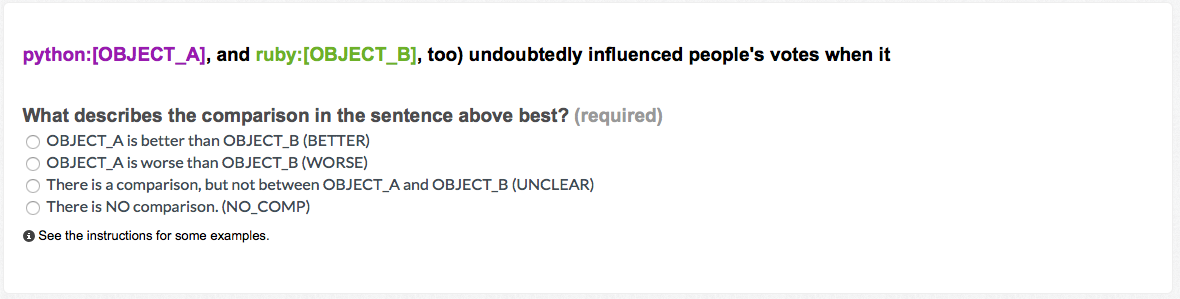
\includegraphics[width=1\textwidth]{images/prestudy/2_question}
\label{img:2_question}
\caption{Annotator view (Prestudy B)}
\end{figure}

The class distribution for the 200 sentences is presentend in figure \ref{fig:dist_pre_b}. 

\begin{figure}[h]
\centering
\caption{Class Distribution (Prestudy B)}
\label{fig:dist_pre_b}
\begin{tikzpicture}
\pie [rotate=180, text = legend, color= {cgray, cgreen, cred, cblue}]
    {48/NO\_COMP (96),
    27/BETTER (54),
    11.5/WORSE (23),
    13.5/UNCLEAR (27)}
\end{tikzpicture}
\end{figure}

As in the first prestudy, nearly half of the sentences are comparative. The agreement (see table \ref{tbl:pre_b_agg}) was better than in the first prestudy. The confusion between \texttt{UNCLEAR} and \texttt{NO\_COMP} is still the main problem for the sentences where only two annotators could agree. However, in the second prestudy this confusion only makes up fourty-five out of the seventy-two cases (62.5\% instead of 87.9\% in the first prestudy). Compared to the first prestudy, the amount of sentences where all annotators agreed on one class increased from 37\% to 62.5\%. Table \ref{tbl:pre_2_res} shows some of the uncertain sentences.

\begin{table}[h]
\caption{Agreement (Prestudy B)}
\label{fig:pre_b_agg}
\begin{tabularx}{\textwidth}{XXX}
\toprule
Distinct classes & Sentences & Percentage \\
\midrule
1 & 125 & 62.50\%\\
2 & 71 & 35.50\%\\
3 & 4 & 2.00\%\\
\bottomrule
\end{tabularx}
\end{table}


\begin{table}[h]
\centering
\caption{Uncertain Sentences (Prestudy B)}
\label{tbl:pre_2_res}
\begin{tabularx}{\textwidth}{lXrrr}
\toprule
\# & Sentence        & Ann. 1  & Ann. 2 & Ann. 3             \\ \midrule
6 & Google shouldn't have mandated an inferior map app on the \textbf{{\color[HTML]{9A14B2}iphone:{[}OBJECT\_A{]}}} (as opposed to \textbf{{\color[HTML]{6CB219}android:{[}OBJECT\_B{]}}}). & BETTER & WORSE & NO\_COMP \\
7 & (See \textbf{{\color[HTML]{9A14B2}android:{[}OBJECT\_A{]}}} Dethrones the \textbf{{\color[HTML]{6CB219} iphone:{[}OBJECT\_B{]}}}.) & BETTER & NO\_COMP & NO\_COMP \\

8 & \textbf{{\color[HTML]{9A14B2}android:{[}OBJECT\_A{]}}} didn't out pace the \textbf{{\color[HTML]{6CB219} iphone:{[}OBJECT\_B{]}}} this year, it just sold slightly better in America & WORSE & NO\_COMP & WORSE\\

9 & To me it is much better than \textbf{{\color[HTML]{9A14B2}iphone:{[}OBJECT\_A{]}}} \mbox{and \textbf{{\color[HTML]{6CB219}android:{[}OBJECT\_B{]}}}}. & NO\_COMP & UNCLEAR & UNCLEAR \\

10 & (\textbf{{\color[HTML]{9A14B2}android:{[}OBJECT\_A{]}}} , Crush , iPad , \mbox{\textbf{{\color[HTML]{6CB219}iphone:{[}OBJECT\_B{]}}}} )& NO\_COMP & BETTER & NO\_COMP \\

\bottomrule                              
\end{tabularx}
\end{table}


From 125 candidate annotators, thirty-five failed the initial quiz. Twelve annotators were removed during the annotation process as they answered too many test questions wrong.

Twenty-two annotators took the exit survey. The overall satisfaction increased to 3.7 out of 5. The test question fairness was now rated with 3.7  instead of 2.9. The rating for the payment slightly increased to 3.9, yet the payment was not changed. However, the rating for the instructions decreased to 3.9 and for the difficulty to 3.5.
The change in numbers is explained by the increased amount of sentences, which introduce new cases which are not directly reflected in the annotation guidelines.
 
\subsection{Validation of results}
Only a small fraction of the annotators took the exit surveys in both prestudies which reduces their explanatory power. However, it gave valuable hints to improve the study design. Yet, the agreement of the annotators is the more important signal.


Using two comparable objects and cue words to query the index returns a satisfiying amount of comparative sentences. Sentence seven (table \ref{tbl:pre_2_res}) shows that it is also benefitial to query the index without cue words. The changes in the second prestudy were well recieved by the annotators. In the end, they improved the quality of results as there are more cases where all three annotators agreed on one class.


The distinction between \texttt{UNCLEAR} and \texttt{NO\_COMP} is still a problem. This illustrates that the choice of a class is subjective to some degree. For instance, sentence five (table \ref{tbl:pre_1_res}) can be understood in two ways. First, one can read it as \emph{PHP is better than OBJECT\_A and OBJECT\_B} because \enquote{\emph{[...] it is so broadly accepted and supported}}. Since those qualities are not mentioned for \texttt{OBJECT\_A} and \texttt{OBJECT\_B}, they can be seen as absent for those objects which makes them worse than PHP. Then, \texttt{UNCLEAR} would be the correct label, because the sentence is comparative but does not compare the objects of interest against each other.

Second, one can read that PHP is an alternative, but there is no expression that it is better, since the sentence does not say it is \emph{more accepted} or \emph{more supported} than \texttt{OBJECT\_A} or \texttt{OBJECT\_B}. In this case, \texttt{NO\_COMP} is the correct class.
\hfill\newline

Due to an error in the creation of the crowdsourcing task, the sentences where not shuffled. This means that the first one-hundred sentences of the second prestudy are the same as the one-hundred sentences of the first prestudy. Another problem is the bias: all sentences contained only the pairs \emph{Ruby vs. Python} and \emph{Android vs. iPhone}. Because the goal of the prestudy was mainly to assess the sentence selection method and the guidelines, this does not invalidate the results. Those problems were removed in the main study.
\hfill\newline

All in all, the prestudy was successful. There are only few cases where no agreement on the class could be achieved. The prestudy showed that the task at hand is not easy, but feasable.

\newpage
\section{Main Study}
\label{sec:mainstudy}
\subsection{Design changes}
The insights from the prestudy influcenced the design of the main study.

The class \texttt{UNCLEAR} was renamed to \texttt{OTHER}, \texttt{NO\_COMP} to \texttt{NONE}. Those names are a better description for the classes. Eventually, after the first 1500 sentences were finished the class \texttt{OTHER} was dropped completly (see section \ref{sec:brands}). The change was reflected in the annotation guidelines as well. 

Instead of one big task, one task per domain was created. All tasks used the same annotation guidelines.


\subsection{Sentence Selection}
The sentence selection process was similar to the prestudy. The pairs and the cue words (see figure \ref{fig:cue_words}) changed. The cue words were generated using JoBimText, a software package for distributional semantics. JoBimText\footnote{http://ltmaggie.informatik.uni-hamburg.de/jobimviz/ (28.02.2018)} was queried for the nine words most similar to \emph{better} and \emph{worse}, so that more, different comparisons are captured by the selection process.

\begin{figure}[h]
\centering
\caption{Cue Words}
\label{fig:cue_words}
\begin{multicols}{4}
better

easier

faster

nicer

wiser

cooler

decent

safer

superior

solid

terrific

worse

harder

slower

poorly

uglier

poorer

lousy

nastier

inferior

mediocre
\end{multicols}
\end{figure}

Three domains were fixed for the object pairs. The domains were chosen in a way that a majority of people can decide whether a sentence contains a comparison or not. Also, a wide range of comparison patterns should be included in the data.

The most specific domain was \enquote{\emph{Computer Science Concepts}}. It contains objects like programming languages, database products and technology standards such as Bluetooth and Ethernet.  Many computer science concepts can be compared objectively, for instance, one can compare Bluetooth and Ethernet on their transmission speed. Some basic knowledge of computer science was needed to label sentences correctly. For example, to compare Eclipse and NetBeans, the annotator must know what an Integrated Development Environment (IDE) is and that both objects are Java IDEs.  The need for this knowledge was communicated to the prospective annotators. The objects for this domain were manually extracted from \enquote{\emph{List of ...}} articles from Wikipedia\footnote{ADD TO APPENDIX}.

The second, broader domain was \enquote{\emph{Brands}}. It contains objects of different types (e.g. car brands, electronics brands, and food brands). As brands are present in everyday life of people, it is expected that anyone can label the majority of sentences containing well known brands such as \enquote{\emph{Coca-Cola}} or \enquote{\emph{Mercedes}}. As with computer science, the objects for this domain were extracted from \enquote{\emph{List of ...}} articles from Wikipedia\footnote{ADD TO APPENDIX}.

The last domain is not restricted to any topic. For each one of twenty-four randomly selected seed words, ten similar words were extracted using JoBimText. The seed words (see figure \ref{fig:seed}) were created using https://randomlists.com\footnote{Last checked: 25.01.2018}. Listing \ref{lst:jbtres} shows the result\footnote{http://ltmaggie.informatik.uni-hamburg.de/jobimviz/ws/api/stanford/jo/similar/harvard\%23NP?numberOfEntries=10&format=json (25.01.2018); Some uninteresting fields were removed for brevity} for the seed word \enquote{\emph{Yale}}. Duplicates or to broad terms (like \emph{university}) were removed by manually.

\begin{figure}[h]
\centering
\caption{Seed words for the Random domain}
\label{fig:seed}
\begin{multicols}{5}
book%23NN

car%23NN

carpenter%23NN

cellphone%23NN

christmas%23NN

coffee%23NN

cork%23NN

florida%23NP

hamster%23NN

hiking

hoover%23NP

metallica%23NP

nbc%23NP

netflix%23NP

ninja%23NN

pencil%23NN

salad%23NN

soccer%23NN

starbucks%23NN

sword%23NN

tolkien%23NP

wine%23NN

wood%23NN

xbox%23NP

yale%23NP
\end{multicols}

\end{figure}

\begin{minipage}{\linewidth}

\begin{lstlisting}[language=json,label=lst:jbtres,caption=Similar words to "Yale"]
[...]
   "results":
      [{"score":701.0,"key":"yale#NP"},
      {"score":245.0,"key":"harvard#NP"},
      {"score":151.0,"key":"princeton#NP"},
      {"score":135.0,"key":"mit#NP"},
      {"score":135.0,"key":"cornell#NP"},
      {"score":121.0,"key":"stanford#NP"},
      {"score":116.0,"key":"university#NP"},
      {"score":111.0,"key":"nyu#NP"},
      {"score":111.0,"key":"university#NN"},
      {"score":109.0,"key":"dartmouth#NP"}]
\end{lstlisting}
\end{minipage}
In the following, this domain is called \emph{Random}. Some example pairs for all domains are shown in table \ref{tbl:exp_pairs}.
\begin{table}[h]
\centering
\caption{Example pairs}
\label{tbl:exp_pairs}

\begin{tabularx}{\textwidth}{XXX}
\toprule
Brands & Computer Science & Random \\
\midrule
Microsoft vs. Apple & Java vs. Python & Baseball vs. Hockey \\
Nikon vs. Leica & Eclipse vs. Netbeans & Fishing vs. Swimming\\
Coca-Cola vs. Pepsi & OpenGL vs. Direct3D & SUV vs. Minivan\\
Nike vs. Adidas & Integer vs. Float & Kennedy vs. Nixon\\
Ibuprofen vs. Advil & USB vs. Bluetooth & Plastic vs. Wood\\
Ford vs. Honda & Oracle vs. MysQL & Harvard vs. Princeton\\

\bottomrule

\end{tabularx}

\end{table}

Especially for brands and computer science, the object lists are long (4493 brands and 1339 for computer science).The frequency of each object was checked using a frequency dictionary to reduce the number of possible pairs. All objects with a frequency of zero and ambiguous objects were removed from the list. For instance, the objects \enquote{\emph{RAID}} (a hardware concept) and \enquote{\emph{Unity}}  (a game engine) were removed from the computer science list as they are also regularly used nouns.

The remaining objects were combined to pairs. For each type, all possible combinations were created. For brands and computer science, the type is the URL of the Wikipedia page. For the random domain, the seed word was used. This procedure guarantees that only meaningful pairs are created.




The index was then queried for entries containing both objects of each pair. For 90\% of the queries, the cue words were added to the query. All pairs were the query yielded at least one-hundred sentences were kept.

From all sentences of those pairs, 2500 for each category were randomly sampled as candidates for the crowdsourcing task. To check the sentence selection method once again, a small, random subset of the sentences was labelled by the author prior to the crowdsourcing task. Those labels were discarded for the crowdsourcing task.
The label distribution of the 742 sentences is presented in the figure \ref{fig:sample}. The numbers are similar to the prestudy which shows that the procedure still works.


\begin{figure}[h]
\centering
\caption{Data precheck}
\label{fig:sample}
\begin{tikzpicture}
\pie [rotate=180, text = legend, sum=100, color= {cgray, cgreen, cred, cblue}]
    {62 /NONE (463),
    17  /BETTER (126),
    8 /WORSE (61),
    13  /OTHER (92)}
\end{tikzpicture}
\end{figure}

\subsection{Brands}
\label{sec:brands}
For the Brands domain, 2493 sentences were annotated. The sentences contained objects of sixty-three pairs. As shown in table \ref{fig:brand_agg}, the annotators could agree on one class for the majority of sentences.

\begin{table}[h]
\caption{Agreement for Brands}
\label{fig:brand_agg}
\begin{tabularx}{\textwidth}{XXX}
\toprule
Distinct classes & Sentences & Percentage \\
\midrule
1 & 1791 & 71.84\%\\
2 & 645 & 25.87\%\\
3 & 57 & 2.29\%\\
\bottomrule
\end{tabularx}
\end{table}



The class distribution is presented in figure \ref{fig:brands_fin}. The amount of comparative sentences is lower (26.1\%) than in the prestudy. The reason for this is the abandonment of the \texttt{OTHER} (\texttt{UNCLEAR}) class. 

\begin{figure}[h]
\centering
\caption{Class distribution for Brands}
\label{fig:brands_fin}
\begin{tikzpicture}
\pie [rotate=180, text = legend, sum=100, color= {cgray, cgreen, cred}]
    {73.9 /NONE (1843),
    18.36  /BETTER (458),
    7.74 /WORSE (193)}
\end{tikzpicture}
\end{figure}



Even with the rephrasing of that class, it was too confusing for the annotators. The class was not different enough from \texttt{NONE} (\texttt{NO\_COMP}). Eventually, all sentences labelled as \texttt{OTHER} (124 sentences for brands) were merged into \texttt{NONE}. This decision was made after 750 sentences were labelled for each domain. First machine learning experiments also showed that \texttt{OTHER} is not distinguishable from \texttt{NONE} for all tested features and algorithms.

For the first 750 sentences, 398 passed the quiz while 357 failed. During the annotation process, fifty-two were removed as they answered to many test questions wrong. The overall satisfaction was 3.4 out of 5. In detail, the acceptance of the task was okay (instructions: 3.9, test question fairness: 3.4, ease of job: 3.4, payment: 3.8).\footnote{The 750 sentences were, due to a mistake, divided into two tasks, one with one-hundred (twenty-six participants in the survey) and one with 650 (fourty-one participants). The presented satisfaction values are the averages weighted by number of participants}

For the rest of the sentences, fifty-one participants took the exit survey. The removal of \texttt{OTHER} increased the overall satisfaction to 3.8 (instructions: 4, test question fairness: 3.5, ease of job: 3.7, payment: 3.7).


\subsection{Computer Science}

For the Computer Science domain, 2465 sentences (containing one of fourty-three pairs) were annotated. As with brands, the agreement of the annotators (table \ref{fig:compsci_agg}) is satisfactory. The class distribution (figure \ref{fig:compsci_fin}) is better, as more sentences are comparative.

\begin{table}[h]
\caption{Agreement for Computer Science}
\label{fig:compsci_agg}
\begin{tabularx}{\textwidth}{XXX}
\toprule
Distinct classes & Sentences & Percentage \\
\midrule
1 & 1757 & 71.28\%\\
2 & 643 & 26.09\%\\
3 & 65 & 2.64\%\\
\bottomrule
\end{tabularx}
\end{table}


\begin{figure}[h]
\centering
\caption{Class distribution for Computer Science}
\label{fig:compsci_fin}
\begin{tikzpicture}
\pie [rotate=180, text = legend, sum=100, color= {cgray, cgreen, cred}]
    {65.64 /NONE (1618),
    23.94  /BETTER (590),
    10.43 /WORSE (257)}
\end{tikzpicture}
\end{figure}

Again, many people failed the quiz (121 failed, 132 passed) for the first 750 sentences. Thirty-five people dropped out during the annotation process because they missed to many test questions. The twenty-seven participants who took the exit survey rated the overall satisfaction with 3.5 (instructions: 3.5, test question fairness: 3, ease of job: 3.2, payment: 3.6).

The numbers improved for the rest of the sentences (after the removal of \texttt{OTHER}). Only sixty-four failed the quiz (379 passed); twenty-six were removed during the annotation process. Fourty-seven participants took the exit survey on the second part. The overall satisfaction was rated with 3.9 (instructions: 4.2, test question fairness: 4, ease of job: 3.8, payment: 3.9).

\subsection{Random}
The random domain has 2463 sentences and 167 pairs. The agreement (table \ref{fig:random_agg}) and class distribution (figure \ref{fig:random_fin}) are satisfactory as well.
    
\begin{table}[h]
\caption{Agreement for Random}
\label{fig:random_agg}
\begin{tabularx}{\textwidth}{XXX}
\toprule
Distinct classes & Sentences & Percentage \\
\midrule
1 & 1766 & 71.70\%\\
2 & 627 & 25.46\%\\
3 & 70 & 2.84\%\\
\bottomrule
\end{tabularx}
\end{table}


\begin{figure}[h]
\centering
\caption{Class distribution for Random}
\label{fig:random_fin}
\begin{tikzpicture}
\pie [rotate=180, text = legend, sum=100, color= {cgray, cgreen, cred}]
    {76.21 /NONE (1877),
    16.24  /BETTER (400),
    7.55 /WORSE (186)}
\end{tikzpicture}
\end{figure}

As with the other domains, the first 750 sentences (with \texttt{OTHER}) performed worse than the rest, as 128 annotators failed the quiz (164 passed) and twenty-seven annotators were removed during the task due to bad performance on the test questions. The Random domain got the worst satisfaction rating (twenty-nine participants) of all domains. The overall satisfaction was rated with 3.1 out of 5 (instructions: 3.6, test question fairness: 3.4, ease of job: 3, payment: 3.4). Once more, the numbers improve after \texttt{OTHER} was removed. Only seventy-five failed the quiz (423 passed). The ratings (thirty-seven participants) increased as well. The overall satisfaction was now rated with 4.0 (instructions: 4.1, test question fairness: 3.9, ease of job: 4, payment: 3.7).


\subsection{Validation of results}

Table \ref{fig:all_agg} summarises the agreement of the annotators on all three domains. The annotators could agree on one class for the majority of the sentences. However, for 28.92\% of the sentences, no clear decision could be made. For 2.67\%, all annotators choose a different class. 

\begin{table}[h]
\caption{Agreement for all}
\label{fig:all_agg}
\begin{tabularx}{\textwidth}{XXX}
\toprule
Distinct classes & Sentences & Percentage \\
\midrule
1 & 5275 & 71.08\%\\
2 & 1948 & 26.25\%\\
3 & 198 & 2.67\%\\
\bottomrule
\end{tabularx}
\end{table}

This shows that the task at hand is difficult even for humans. For instance, sentence one in table \ref{tbl:all_res} requires knowledge on mobile phones to be classified correctly. It also lacks a cue word. Sentence five includes a cue word (\emph{harder}) and \emph{than} which make it look like a comparison. However, the sentence is not a comparison in a way that one object wins against the other. In sentence two, the annotators overlooked the negation (\enquote{\emph{wouldn't}}).

\begin{table}[h]
\centering
\caption{Uncertain Sentences (All)}
\label{tbl:all_res}
\begin{tabularx}{\textwidth}{lXrrr}
\toprule
\# & Sentence        & Ann. 1  & Ann. 2 & Ann. 3             \\ \midrule
1 & \textbf{{\color[HTML]{9A14B2}Samsung:{[}OBJECT\_A{]}}} voids warranty for rooting, \textbf{{\color[HTML]{6CB219}Motorola:{[}OBJECT\_B{]}}} doesn't. & NONE & WORSE & BETTER\\
2 & I wouldn't say \textbf{{\color[HTML]{9A14B2}Microsoft:{[}OBJECT\_A{]}}} is worse then \textbf{{\color[HTML]{6CB219}Apple:{[}OBJECT\_B{]}}}. & NONE & WORSE & WORSE\\

3 & If you use \textbf{{\color[HTML]{9A14B2}NetBeans:{[}OBJECT\_A{]}}} instead of \textbf{{\color[HTML]{6CB219}Eclipse:{[}OBJECT\_B{]}}} & OTHER & BETTER & NONE \\
4 & Visibly faster than \textbf{{\color[HTML]{9A14B2}Python:{[}OBJECT\_A{]}}} ... faster than \textbf{{\color[HTML]{6CB219}Java:{[}OBJECT\_B{]}}} I'd bet. & NONE & BETTER & BETTER \\
5 & It's light as \textbf{{\color[HTML]{9A14B2}aluminum:{[}OBJECT\_A{]}}}, but harder than \textbf{{\color[HTML]{6CB219}steel:{[}OBJECT\_B{]}}}, he said. & NONE & OTHER & BETTER\\
\bottomrule                              
\end{tabularx}
\end{table}


The class distribution (figure \ref{fig:all_fin}) is similar to the prestudy. As expected, the majority of sentences is not comparative. 
The class \texttt{BETTER} is more than twice as big as the class \texttt{WORSE}, which will complicate the classification.
\begin{figure}[h]
\centering
\caption{Class distribution for all}
\label{fig:all_fin}
\begin{tikzpicture}
\pie [rotate=180, text = legend, sum=100, color= {cgray, cgreen, cred}]
    {71.92 /NONE (5338),
    19.51  /BETTER (1448),
    8.57 /WORSE (636)}
\end{tikzpicture}
\end{figure}

In the end, the crowdsourcing task was successful. For the majority of sentences (71.08\%) the annotators could agree on one class, while the amount of totally unclear sentences is small (2.67\%).